\section{Accepttest}
Der kan ses ud fra målingerne at frekvensgangen ved 2 V, afbilledet på figur \ref{fig:acceff:frek2v}, ved de lave frekvenser, ikke er tilfredsstillende. Da frekvensgangen for 2 V og 200 mV bedømmes til at være meget ens, konkluderes der kun på frekvensgangen for 2 V.

\begin{figure}[h]
\centering
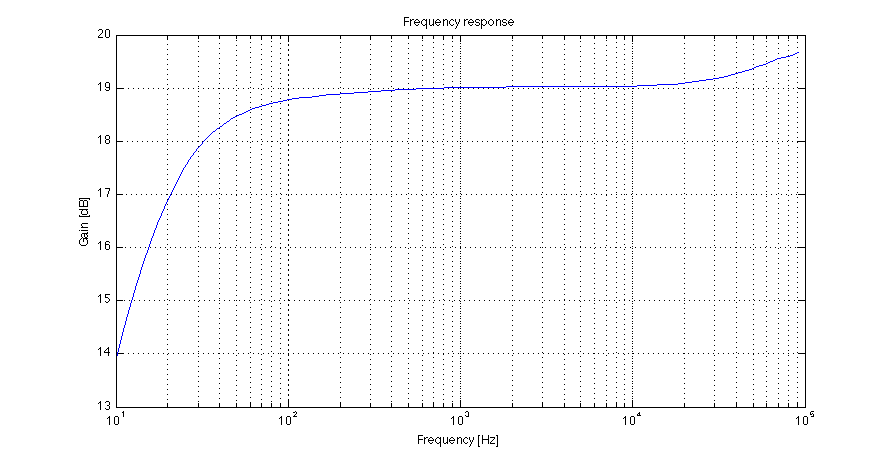
\includegraphics[width=\textwidth]{maalerapporter/effektforstaerker/2V-45mA-uden-modstand-frek.png}
\caption{Den målte frekvensgangen for effektforstærkeren ved 2 V}
\label{fig:acceff:frek2v}
\end{figure}

Ved 20 Hz aflæses forstærkningen til 17 dB, mens forstærkningen ved 63 Hz aflæses til 18,6 dB. Dette er en forskel på 1,6 dB, hvilket er mere end de 0,75 dB den skulle være indenfor. Forstærkningen ved 1 kHz er aflæst til 19 dB. Forskellen til de 63 Hz er ca. 0,4 dB, hvilket er tæt på de krævede 0,375 dB men ikke acceptabelt. Forstærkningen ved 12 kHz aflæses til 19,1 dB, mens forstærkningen ved 20 kHz aflæses til 19,3 dB. Denne afvigelse på 0,2 dB er under kravet på 0,75 dB, hvilket derfor er acceptabelt.

Afvigelsen fra kravet om dæmpningen fra 20 Hz til 63 Hz skyldes sandsynligvis at kondensatorudregningen for lavpasfilteret i tilbagekoblingen er forkert. Hvis kondensatoren havde været større, havde polens knækfrekvens været flyttet ned i frekvens, hvilket ville have dæmpet de lave frekvenser mindre, da knækket ikke ville have været betydeligt til stede ved de relevante frekvenser. Grundet tidsmangel er dette dog ikke opfanget under simuleringen og blev derfor først opdaget under implementeringen.

På figur \ref{fig:acceff:thd2v} ses THD-målingen af effektforstærkeren. Målingen for 2 V er valgt, da denne giver de største værdier og derfor danner grundlag for at bedømme om THD'en holder sig under det ønskede. 
\begin{figure}[h]
\centering
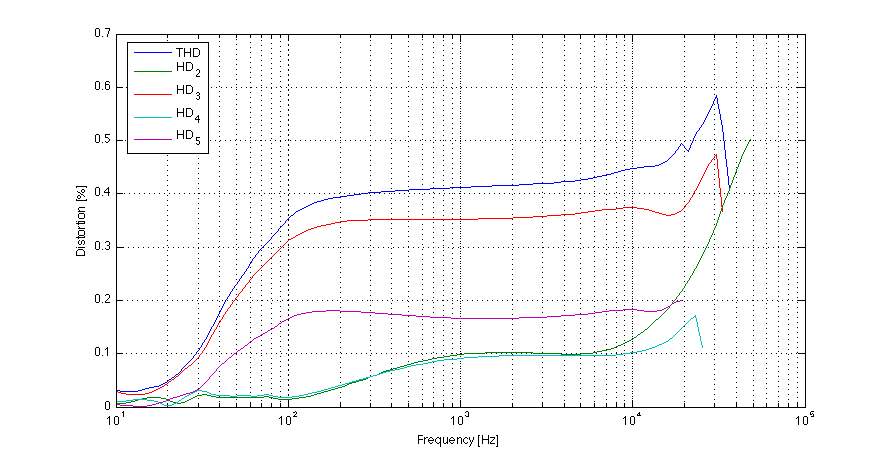
\includegraphics[width=\textwidth]{maalerapporter/effektforstaerker/2V-45mA-uden-modstand-thd.png}
\caption{Den målte THD for effektforstærkeren ved 2 V}
\label{fig:acceff:thd2v}
\end{figure}

Der kan aflæses at THD ved fuld udstyring når et maksimum på 0,49 \%, ved 19 kHz. Dette er under de 0,5\% der er defineret som et krav og er derfor accepteret. 

Nyttevirkningen er, i Appendiks \ref{maalejournal-effekt}, målt til 53 \% ved maksimal udstyring og 1 kHz, hvilket er acceptabelt da den, ifølge kravspecifikationen skal ligge mellem 25 og 78,5 \%. \fixme{Skriv om nyttevirkning i appendiks!}



\begin{table}[h]
\centering
\begin{tabular}{l|c|r}
\hline\hline
Område & Krav & Status\\
\hline\hline
Indgangsimpedans & 22 k\ohm & Opfyldt \\[4pt]
Frekvensgang & $\pm$ 0,375 dB ved 20 Hz - 20 kHz, ref. 1 kHz & Opfyldt \\
& $\pm$ 0,75 dB fra 20 Hz til 63 Hz & Opfyldt\\
& $\pm$ 0,75 dB fra 12,5 kHz til 20 kHz & Opfyldt\\[4pt]
Forvrængning & < 0,5 \% & Opfyldt\\[4pt]
Forstærkning & 69,7 gange ved 22 k\ohm~ indgangsimpedans og ved 1 kHz & Opfyldt\\
\hline\hline
\end{tabular}
\caption{Krav til forforstærkeren}
\label{tab:krav_forforstaerker}
\end{table}